% !TeX program = pdflatex
% REF-001, IEEE conference-format research draft.
% Replace the author placeholder with the confirmed author list and affiliations.
\documentclass[conference]{IEEEtran}

\usepackage{cite}
\usepackage{amsmath}
\usepackage{booktabs}
\usepackage{tabularx}
\usepackage{tikz}
\usetikzlibrary{arrows.meta,positioning}
\usepackage[hidelinks]{hyperref}

\title{Evidence-Grounded Housing Transaction Comparison in Taiwan Using a Bounded ReAct Agent}

\author{\IEEEauthorblockN{Author information pending}
\IEEEauthorblockA{National Chung Hsing University\\Taichung, Taiwan}}

\begin{document}
\maketitle

\begin{abstract}
Taiwan's public real-estate transaction records enable residential price comparison, but differences in property type, transferred area, and parking treatment complicate the interpretation of prices. We propose a housing intelligence agent that combines bounded reasoning and acting (ReAct), retrieval-augmented generation, and deterministic transaction analytics. The agent uses approved read-only tools and attaches claim-level evidence, including data versions, calculation rules, and applicable dates. An evidence gate validates tool outputs and withholds price claims when supporting transaction evidence is unavailable. A preliminary project audit examined one Taichung City release with 10,638 records and 32 fields. An exploratory filter retained 9,152 residential candidates, supporting further investigation of field definitions and residential eligibility. The planned evaluation compares adaptive tool selection with a fixed workflow using identical tools and evidence. Its outcomes include supported task completion, citation support, appropriate abstention, latency, and resource use. The snapshot audit is the empirical work reported here. Agent implementation and comparative evaluation are planned.
\end{abstract}

\begin{IEEEkeywords}
housing transactions, ReAct, data provenance, decision support
\end{IEEEkeywords}

\section{Introduction}
Public transaction records help housing buyers identify comparable sales and examine how observed prices vary across locations and property types. A sale with a separately priced parking space and a sale with a bundled parking price can look comparable even though their price and area fields describe different transfer bundles. Taiwan's Ministry of the Interior (MOI) documents these reporting conventions and explains that the public service excludes some exceptional transactions \cite{moi}. A useful comparison therefore needs a declared sample definition and price convention alongside the reported numbers.

Consider a request to compare residential towers in two districts over the same period. The system must resolve the districts, select a common price definition, retrieve comparable cohorts, and explain exclusions. It may also need to check which version of a data definition applied at a particular date. An answer can appear plausible while using different parking adjustments in each district or comparing cohorts with unequal time coverage. Retrieving the relevant documents and producing the numerical summary are separate operations, and both require evidence.

We propose a bounded agent for descriptive housing comparison. Taichung is the candidate study area. The final definition of eligible existing homes depends on source coverage and confirmed field semantics. The primary research question is whether adaptive tool selection improves supported task completion on conditional and multi-step housing queries when a fixed workflow has access to the same tools and evidence. The study also asks how each approach handles cases in which only part of a question can be answered.

The proposed design includes an evidence contract for numerical and documentary claims, a response policy for missing or conflicting evidence, and a paired evaluation protocol. Section~\ref{sec:related} reviews housing analytics and tool-using agents. Sections~\ref{sec:data} and~\ref{sec:method} describe the preliminary audit and architecture. Section~\ref{sec:evaluation} specifies the evaluation.

\section{Related Work}
\label{sec:related}
\subsection{Housing Analytics and Spatial Evidence}
Wang \emph{et al.} combine transaction attributes, public-facility information, and satellite imagery in a price prediction model evaluated on historical Taipei and New Taipei sales \cite{wang}. Their study motivates the conditional use of location features when source quality and spatial precision support the task. Descriptive comparison starts from a different question about the observed distribution within an explicitly filtered cohort. Its interpretation depends on reproducible eligibility criteria and consistent price and area definitions.

Roberts \emph{et al.} discuss how temporal and spatial dependence affect validation and recommend aligning the separation of training and test data with the intended prediction setting \cite{roberts}. We apply this principle to possible valuation work by holding out future transactions and considering geographic transfer only where coverage supports it. Lundberg and Lee's SHAP method attributes fitted model predictions to input features \cite{shap}. Attribution, predictive accuracy, and a user's understanding of an answer are distinct outcomes in the proposed evaluation.

\subsection{Tool-Using Agents}
ReAct interleaves reasoning, actions, and observations so that an external result can inform the next action \cite{react}. Retrieval-augmented generation (RAG) conditions generation on retrieved information \cite{rag}. Haurum \emph{et al.} demonstrate the use of a LangChain-based agent for real-estate information \cite{haurum}. Our study examines whether adaptive orchestration changes the evidence support of answers when the controller and a predefined workflow share the same data and tool contracts.

The proposed agent uses ReAct for orchestration and RAG for domain-document retrieval. It draws numerical claims from structured tools with explicit calculation rules. Documentary claims require an applicable source version and passage. This division makes it possible to trace a price statistic back to the queried snapshot and to check whether cited documentary evidence was valid for the requested time and jurisdiction.

\section{Data and Preliminary Feasibility}
\label{sec:data}
\subsection{Observed Snapshot Audit}
The project team's exploratory audit used the Taichung City Land Administration Bureau sales CSV labeled July--September of ROC year 115 (2026) under dataset 103038 \cite{taichung}. The exploratory filter retained \emph{land and building} and \emph{land, building, and parking} transactions belonging to four selected building types. Parsing the official CSV and reapplying those category filters reproduced the audit counts in Table~\ref{tab:snapshot}. The retained subset comprises 86.0\% of the release. Its share describes the effect of the filter on the published records.

\begin{table}[t]
\caption{Observed Counts Reported in the Single-Snapshot Audit}
\label{tab:snapshot}
\centering
\begin{tabularx}{\columnwidth}{@{}Xr@{}}
\toprule
Audit item & Count \\
\midrule
Raw records & 10,638 \\
Source fields & 32 \\
Residential candidates & 9,152 \\
\quad Elevator buildings, 11 floors or more & 5,933 \\
\quad Elevator buildings, 10 floors or fewer & 1,553 \\
\quad Townhouses & 1,461 \\
\quad Walk-up apartments, 5 floors or fewer & 205 \\
\bottomrule
\end{tabularx}
\end{table}

The quarter is the publication batch label. The business meaning of the encoded ROC year-month field remains unconfirmed for this extract, so the audit cannot establish transaction-quarter coverage. The team classified the snapshot as conditionally feasible for further schema and eligibility review. Historical coverage, the final study population, and any supervised prediction target remain open. The reported counts give no estimate of agent reliability or model accuracy.

\subsection{Cohort Construction and Price Conventions}
The proposed ingestion process records the source URL, release identifier, retrieval time, checksum, and schema version. The query records the exact inclusion predicate and transformation version. Before enabling a period-based comparison, the team will verify the data dictionary and distinguish transaction dates from registration and publication dates wherever the corresponding fields exist. The data audit will check missing values, possible duplicates, parking fields, and coverage by district and building type. It will document the effect of each eligibility rule on the count.

For a parking-excluded comparison, let \(P_i\) denote the reported transfer price in New Taiwan dollars and \(A_i\) the compatible transfer area in square metres. Let \(P_{i,p}\) and \(A_{i,p}\) denote the separately reported parking price and area. The proposed rule is
\begin{equation}
u_i = \frac{P_i-P_{i,p}}{A_i-A_{i,p}},
\qquad A_i>A_{i,p}.
\label{eq:unitprice}
\end{equation}
The rule applies only when the components use compatible source definitions and satisfy the schema and validity checks. For a confirmed sale without parking, both parking components are zero. A sale with a missing required component is excluded from the parking-adjusted metric and may enter a separately labeled bundled-price analysis if eligible. If a comparison instead uses a source-provided unit price, the response identifies that field and the source's parking convention \cite{moi}.

For an eligible cohort, the descriptive tool reports the sample count and, where support permits, the median and interquartile range. The median summarizes the per-record unit prices computed using \eqref{eq:unitprice}. The MOI's aggregate average divides summed prices by summed areas \cite{moi}. The response names the statistic and provides the metric definition, units, applicable period, and exclusion count. A minimum support rule, to be fixed before the evaluation, determines when a cohort is too sparse to report a numerical result.

\section{Proposed System}
\label{sec:method}
\begin{figure}[t]
\centering
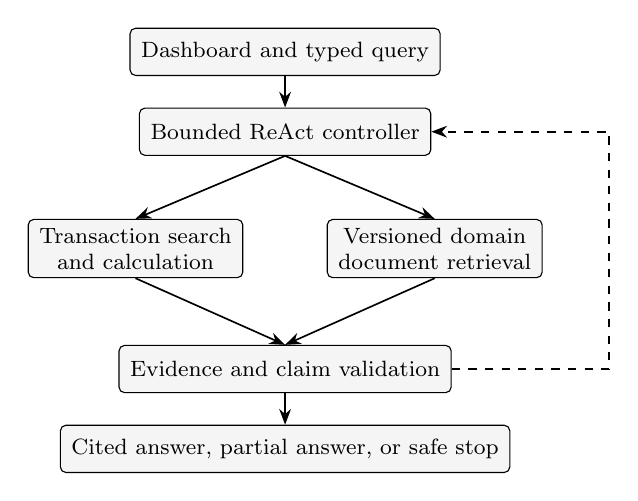
\begin{tikzpicture}[
  block/.style={draw, rounded corners=2pt, align=center, font=\footnotesize,
    minimum height=6mm, inner xsep=4pt, inner ysep=3pt, fill=black!4},
  edge/.style={-{Stealth[length=2mm]}, semithick},
  node distance=4mm]
  \node[block] (query) {Dashboard and typed query};
  \node[block, below=of query] (agent) {Bounded ReAct controller};
  \node[block, below=8mm of agent, xshift=-19mm] (data) {Transaction search\\and calculation};
  \node[block, below=8mm of agent, xshift=19mm] (rag) {Versioned domain\\document retrieval};
  \node[block, below=24mm of agent] (gate) {Evidence and claim validation};
  \node[block, below=of gate] (answer) {Cited answer, partial answer, or safe stop};
  \draw[edge] (query) -- (agent);
  \draw[edge] (agent.south) -- (data.north);
  \draw[edge] (agent.south) -- (rag.north);
  \draw[edge] (data.south) -- (gate.north);
  \draw[edge] (rag.south) -- (gate.north);
  \draw[edge] (gate) -- (answer);
  \draw[edge,dashed] (gate.east) -- ++(20mm,0) |- (agent.east);
\end{tikzpicture}
\caption{Proposed control and evidence flow. The dashed path returns a validated observation to the controller.}
\label{fig:architecture}
\end{figure}

\subsection{Typed Query and Bounded Orchestration}
Fig.~\ref{fig:architecture} shows the control flow. The parser converts a natural-language question into a typed request containing the comparison intent, district, period, property type, attributes, and applicable date where needed. An unclear district or price convention can trigger a clarification request. The design allows up to two clarification rounds. Scope checks also identify requests that require evidence or capabilities outside the project.

The controller takes up to six ReAct steps per request. Before execution, each proposed action must match an approved read-only tool and supply valid typed arguments. A transient failure permits one retry of the affected call. When a core source is invalid or unavailable, the controller can select an approved alternative within its budget. A trace records selected tools, validated arguments, source versions, observation status, and the response decision. The trace limits the retention of personal and fine-grained location data.

\subsection{Evidence Contracts and Validation}
A transaction observation includes the snapshot identifier, sample predicate, schema version, calculation version, output units, and quality flags. The output associates each statistic with its eligible sample. The response layer copies numbers from valid tool outputs and associates each with the metadata required to reproduce the calculation.

A domain observation includes the source authority, document identifier and passage, version, jurisdiction, publication or effective dates, and applicability conditions. Retrieval uses the requested as-of date. The design distinguishes regulatory facts, market evidence, expert opinion, and hypotheses in the source registry. A topically relevant document may fail the applicability check because a newer version supersedes it or its jurisdiction or property category differs from the query.

The evidence gate applies the checks in Table~\ref{tab:gate}. Invalid, stale, or inapplicable results are excluded from computation and claim generation. Before a response is shown, each displayed number must match a validated output and each documentary claim must be supported by an applicable passage. Separately supported findings can be returned with an explanation of the missing evidence. When all authorized core sources fail validation, the response withholds the price claim and explains the reason.

\begin{table}[t]
\caption{Proposed Evidence Checks and Response Behavior}
\label{tab:gate}
\centering
\small
\begin{tabularx}{\columnwidth}{@{}>{\raggedright\arraybackslash}p{.30\columnwidth}>{\raggedright\arraybackslash}X@{}}
\toprule
Check & Behavior when evidence fails \\
\midrule
Authorization and arguments & Reject the proposed tool call before execution. \\
Schema, units, or provenance & Exclude the result from calculations and claims. \\
Version, date, or applicability & Withhold the affected claim and disclose the omission. \\
Core transaction evidence & Check an authorized alternative within budget. Withhold prices when valid evidence is unavailable. \\
Optional GIS or model output & Omit that output and retain independently supported transaction findings. \\
\bottomrule
\end{tabularx}
\end{table}

\subsection{Illustrative Query}
Suppose a user requests the median parking-excluded unit price for residential towers in two Taichung districts over a specified period. After validation, the system identifies the two cohorts using the same snapshot and metric. If one district has adequate support and the other has too few eligible records with separate parking fields, the dashboard can show the supported district summary and identify the missing evidence. If neither cohort can support a price, the dashboard returns the eligibility or coverage issue without a numerical finding. Controlled records will be used to test this expected behavior.

\subsection{Design Trade-offs}
Adaptive tool selection may recover from an unusable source or retrieve documents only when needed. This flexibility consumes resources and can introduce inconsistent decisions. The shared evidence policy and the fixed workflow make those costs measurable. Optional valuation introduces additional error and explanation requirements. Optional geographic information system (GIS) features depend on approved use, location precision, coordinate references, and geographic coverage. When those conditions are unmet, the comparison remains at the supported aggregation level.

\section{Planned Evaluation}
\label{sec:evaluation}
\subsection{Data and Analytics Evaluation}
The first stage verifies the date and area fields, historical coverage, source permissions, and residential inclusion rules. Evaluators will independently reconstruct reference cohort counts and statistics from frozen snapshots. Test cases will include missing parking components, invalid adjusted area, and sparse cohorts. The evaluation will measure numerical agreement under a common rounding rule and the correctness of inclusion and exclusion decisions.

If eligible historical data and a defensible target are available, a secondary experiment will compare an area-and-time median baseline, a linear model, and a tree-based model using a common target and feature availability rules. Training data precede the held-out period. Preprocessing, aggregate features, and tuning use only training data. A spatial holdout will be considered where geographic transfer matches the intended use and the data support it. Planned measures include mean absolute error, root mean squared error, \(R^2\), and errors by property type and geographic subgroup. A model output would be exposed only for inputs inside its validated scope.

\subsection{Paired Agent Evaluation}
The fixed workflow follows a predefined sequence with conditional branches for clarification, retrieval, and failure. The adaptive workflow allows the bounded ReAct controller to select the next step based on validated observations. Both arms share the task inputs, query parser, data and document versions, available tools, audit policy, and response requirements. Where the arms use a language model for query interpretation or answer assembly, those shared tasks use the same model and settings. The evaluation also applies the same request resource limits to both arms.

The paired task set will include routine district comparisons, ambiguous questions, stale or conflicting documents, transient failures, missing core records, and invalid optional outputs. The reference for each case specifies the expected decision, necessary evidence, acceptable caveats, and claims that must be withheld. Appropriate clarification and safe stops can count as successful task completion. Results will be stratified by routine, multi-step, and failure cases to identify where the choice of controller matters.

The evaluation will freeze the task set and scoring rubric before the test runs. Cases involving transient failures or contradictory documents will use controlled fixtures so that both workflows encounter equivalent evidence conditions. Reviewers will score the final responses against the reference without seeing which workflow produced them. They will resolve disagreements against the underlying tool outputs and source passages. Execution traces will be scored separately to identify failures that the final answer alone cannot reveal.

Citation support is the fraction of auditable claims whose cited evidence supports their content and scope. The report will give claim counts alongside this measure and separately count responses with unsupported price claims. Among cases whose reference requires withholding a price, we will measure correct abstention. Among answerable cases, we will measure unnecessary abstention. Tool traces will be checked for invalid arguments, unauthorized actions, and violations of step and retry limits. Efficiency measures include median and 95th-percentile latency, calls per query, and model token use under common execution conditions.

The analysis will report paired differences and uncertainty intervals from resampling task cases, grouping variants derived from the same template. If the controller is stochastic, repeated runs will retain their case identifiers so that repetitions are analyzed within a case. A separate comprehension study, if feasible, will assess whether readers can identify the comparison period, explain the price convention, and distinguish a disclosed-sample statistic from a property-level estimate.

\section{Limitations and Conclusion}
The audit covers one municipal release and exploratory residential categories. Its distribution depends on disclosure, release composition, and the team's filtering rules. The release does not establish population representativeness or temporal generalizability. Fine-grained GIS depends on consistent geographic linkage and approved location precision. Version metadata supports the review of documentary evidence, while some applicability questions may still require qualified interpretation. The intended use is informational comparison of disclosed sales. Individual appraisal and personalized financing, tax, or investment recommendations fall outside the study scope.

The proposed agent connects a typed housing query to a documented snapshot, a deterministic calculation, and a verifiable final claim. The observed Taichung audit supports further feasibility work and identifies questions about date semantics and eligibility. Confirming field definitions and executing the paired workflow study will make it possible to estimate when adaptive orchestration improves supported task completion and how much time and resource use it adds.

\begin{thebibliography}{00}
\bibitem{moi}
Ministry of the Interior, Taiwan, \textquotedblleft Real estate transaction price inquiry service: Frequently asked questions.\textquotedblright\ [Online]. Available: \url{https://lvr.land.moi.gov.tw/jsp/qa.jsp}

\bibitem{wang}
P.-Y. Wang, C.-T. Chen, J.-W. Su, T.-Y. Wang, and S.-H. Huang, \textquotedblleft Deep learning model for house price prediction using heterogeneous data analysis along with joint self-attention mechanism,\textquotedblright\ \emph{IEEE Access}, vol. 9, pp. 55244--55259, 2021, doi: 10.1109/ACCESS.2021.3071306.

\bibitem{roberts}
D. R. Roberts \emph{et al.}, \textquotedblleft Cross-validation strategies for data with temporal, spatial, hierarchical, or phylogenetic structure,\textquotedblright\ \emph{Ecography}, vol. 40, no. 8, pp. 913--929, 2017, doi: 10.1111/ecog.02881.

\bibitem{shap}
S. M. Lundberg and S.-I. Lee, \textquotedblleft A unified approach to interpreting model predictions,\textquotedblright\ in \emph{Advances in Neural Information Processing Systems}, vol. 30, 2017.

\bibitem{react}
S. Yao, J. Zhao, D. Yu, N. Du, I. Shafran, K. Narasimhan, and Y. Cao, \textquotedblleft ReAct: Synergizing reasoning and acting in language models,\textquotedblright\ in \emph{Proc. Int. Conf. Learn. Representations}, 2023.

\bibitem{rag}
P. Lewis \emph{et al.}, \textquotedblleft Retrieval-augmented generation for knowledge-intensive NLP tasks,\textquotedblright\ in \emph{Advances in Neural Information Processing Systems}, vol. 33, pp. 9459--9474, 2020.

\bibitem{haurum}
K. R. Haurum, R. Ma, and W. Long, \textquotedblleft Real estate with AI: An agent based on LangChain,\textquotedblright\ \emph{Procedia Comput. Sci.}, vol. 242, pp. 1082--1088, 2024, doi: 10.1016/j.procs.2024.08.199.

\bibitem{taichung}
Taichung City Land Administration Bureau, \textquotedblleft Taichung real estate transaction price registration: Sales since ROC year 110,\textquotedblright\ Taiwan Government Open Data Platform, dataset 103038. [Online]. Available: \url{https://data.gov.tw/dataset/103038}
\end{thebibliography}

\end{document}
